\section{Decisions at a positive error tolerance}
\label{sec:decision-value}

\paragraph{Decisions in the KAHM forecasting studies.}
The main synthetic, oscillator, and coefficient-budget studies contain 62
fitting runs (Sections~\ref{sec:experiments}--\ref{sec:budget-sensitivity}).
We distinguish exclusion of a candidate's decoder class from the behavior
of a model selected by validation. Among the 800 main-study candidates, the all-horizon decisions at
RMSE tolerance $0.35$ are 301 accepted, 24 excluded, and 475 unresolved;
the corresponding oscillator counts are 55, 30, and 155 among 240 candidates.
Nevertheless, all 186 horizon-specific lower endpoints of the 62 models
selected by validation across the complete candidate family are zero.
Restricting validation selection to retained KAHM gives 184 zero endpoints
out of 186. These descriptive counts motivate a separate test of whether
lower certificates can resolve a decision that upper calibration leaves open.

\paragraph{A controlled forecasting mechanism.}
The protocol is specified before calibration observations are generated.
Each independent episode supplies one history $X=(Z,S)$ and one scalar future
$Y$. The indicator $S$ equals one with probability $0.2$ and zero otherwise,
and $Z,R,N$ are mutually independent random signs, each taking $-1$ and $1$
with equal probability, independently of $S$. We consider two regimes, called
repairable and irreducible because the final
representation can remove the signal uncertainty only in the first:
\[
  Y=0.8SZ+0.1N \quad\text{(repairable)},\qquad
  Y=0.8SR+0.1N \quad\text{(irreducible)}.
\]
The three entries of $(Z,S,Y)$ occur in temporal order, and the forecast is
made after observing $Z$ and $S$, before observing $Y$. The target range is
$[-0.9,0.9]$. We append the simplex
blocks
\[
 (1),\qquad (1-S,S),\qquad
 \bigl((1+SZ)/2,(1-SZ)/2\bigr)
\]
under the common coefficient budget $\kappa=2$. The first block has one
coordinate; the first two have three coordinates in
total; and all three have five. These coordinate counts define the costs
$1,3,5$ of the three representation classes. These explicit representations
test the general theorem; they are not fitted KAHM dictionaries.

At costs $1$, $3$, and $5$, the exact minimum MSEs in the repairable regime
are $0.138$, $0.138$, and $0.01$. They all equal $0.138$ in the irreducible
regime. In the former, the last
block represents the conditional mean $0.8SZ$ with coefficients
$(0.8,-0.8)$, whose norm is below $2$. In the latter, the unobserved sign $R$
leaves the conditional mean zero even with the complete history. The prescribed
RMSE tolerance $0.30$ therefore requires the last prefix in one regime and
is unattainable in the other. For the cost-$3$ prefix, the unconditional
population witness is only $0.0324$, whereas pairing conditionally on $S$
gives $0.138$. This isolates a population limitation of unconditional pairing,
in addition to finite-sample uncertainty.

\paragraph{Calibration and comparisons.}
Each of 100 independent repetitions per regime uses 2,048 training episodes,
1,024 validation episodes, and nested calibration samples of
$256,1024,4096,16384,65536$ episodes. All three decoders are fitted with zero
ridge penalty and frozen before calibration. The RMSE tolerance $0.30$
corresponds to an MSE threshold of $0.09$. We compare validation-only
acceptance at this threshold, calibrated upper-bound acceptance, and two
extensions of the latter rule using either unconditional or stratified
lower certificates.
Validation-only acceptance is a descriptive reference rule without a population
confidence guarantee. The two predefined partitions use the history labels
$S$ and $(S,Z)$; neither
partition uses the future target. For the latter method, we estimate
stratum masses and take the maximum of the two separately budgeted endpoints
from Theorem~\ref{thm:stratified-certificate}. One failure budget $0.05$ per
regime and repetition covers all prefixes and all five sample sizes:
$0.02$ for upper bounds, $0.01$ for unconditional lower bounds, and $0.02$
for both stratified families. Calibration uses one forecast per independent
episode; it does not treat dependent windows as independent observations.

\begin{table}[t]
\centering
\small
\begin{tabular}{rccccc}
\toprule
 & \multicolumn{3}{c}{Repairable regime} & \multicolumn{2}{c}{Irreducible regime} \\
\cmidrule(lr){2-4}\cmidrule(lr){5-6}
$n$ & Upper & \multicolumn{2}{c}{Minimum cost $5$} & \multicolumn{2}{c}{All classes excluded} \\
 & acceptance & Unconditional & Stratified & Unconditional & Stratified \\
\midrule
256 & 0 & 0 & 0 & 0 & 0 \\
1,024 & 100 & 0 & 0 & 0 & 0 \\
4,096 & 100 & 0 & 0 & 0 & 0 \\
16,384 & 100 & 0 & 100 & 0 & 1 \\
65,536 & 100 & 0 & 100 & 0 & 100 \\
\bottomrule
\end{tabular}
\caption{Decision counts out of 100 independent repetitions in each constructed regime, at the prespecified RMSE tolerance $0.30$. Upper acceptance certifies a fitted predictor; equality of the cost endpoints certifies the least feasible cost among the three predefined classes. The unconditional and stratified methods share the same upper endpoint and fitted model. Every irreducible-regime upper decision is unresolved. One failure budget $0.05$ covers all five calibration sizes and all reported endpoints within each regime and repetition.}
\label{tab:decision-outcomes}
\end{table}


\paragraph{Decision value and sample requirements.}
Validation accepts the repaired cost-$5$ model in all 100 repetitions, and
upper calibration does so from $n=1024$ onward. Stratified lower certificates
exclude both cheaper classes in all repetitions at $n=16384$ and $65536$,
so the cost interval in Corollary~\ref{cor:cost-optimality} reduces to
$[5,5]$. Unconditional lower calibration never closes this interval at the
prescribed sample sizes. Both procedures select the same accepted predictor;
the additional conclusion is that no cheaper prescribed class can meet the
tolerance, independently of its decoder optimization.

The irreducible control produces no upper acceptance. Stratified lower
calibration excludes all three classes in 1 of 100 repetitions at $n=16384$
and all 100 at $n=65536$; unconditional lower calibration never excludes all
three. Small samples reveal the cost of stratification: at $n=4096$,
unconditional pairing excludes the constant class in every repetition of
both regimes, while the stratified method excludes no class. All 600 fits
converged, and the exact population risks satisfy every reported simultaneous
interval event in all 200 regime--repetition instances. The experiment
demonstrates a class-level decision under a controlled mechanism, with
substantial sample requirements; it does not establish its frequency in
natural forecasting tasks.

\begin{figure}[t]
\centering
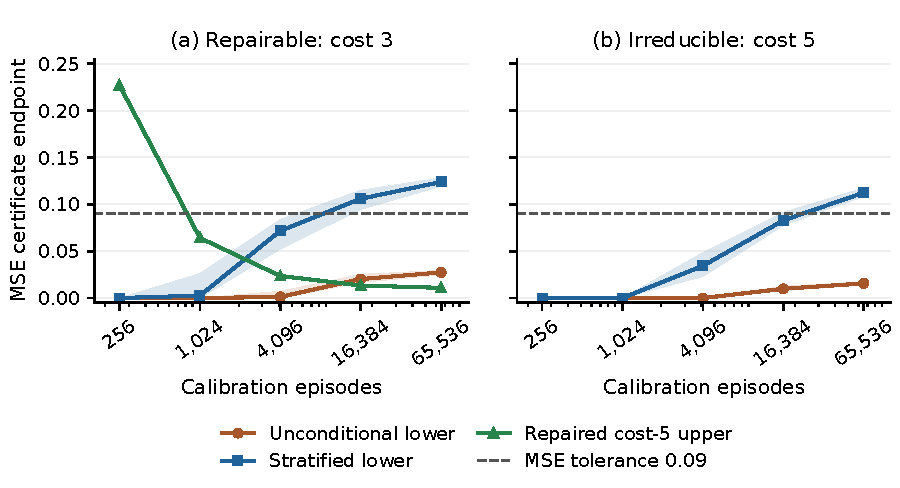
\includegraphics[width=\linewidth]{figures/decision_endpoints.pdf}
\caption{Calibration-size dependence in the constructed decision experiment.
Lines show medians and shaded bands the full range across 100 independent
repetitions; the bands describe repetition variability. Panel (a) compares
lower endpoints for the inadequate cost-$3$ class with the upper endpoint
for the repaired cost-$5$ predictor. Panel (b) shows lower endpoints for the
most detailed class in the irreducible regime. The dashed line is the fixed
MSE tolerance $0.09$.}
\label{fig:decision-endpoints}
\end{figure}
